\documentclass[12pt,a4paper]{article}
\usepackage[utf8]{inputenc}
\usepackage{amsmath}
\usepackage{amsfonts}
\usepackage{amssymb}
\usepackage{enumerate}
\usepackage[T1]{fontenc}
\usepackage{graphicx}
\usepackage{polski}

\usepackage{array}
\title{Projekt SINGIEL 2.0}
\newcolumntype{l}{m{185pt}}
\begin{document}
\begin{center}
Państwowa Wyższa Szkoła Zawodowa w Nowym Sączu
\end{center}

\begin{center}
Projekt SINGIEL 2.0
\end{center}
\newpage

\section{Temat:}
Aplikacja randkowa z komunikatorem.
\section{Nazwa:}
SINGIEL 2.0
\section{Opis cel i zakres pracy:}

SINGIEL 2.0 to aplikacja pełna możliwości. Możemy zawierać znajomości poprzez parowanie się użytkowników. Jeśli chcesz poszerzyć krąg towarzyski, spotkać się z kimś i poznawać nowych ludzi to znajdujesz się we właściwym miejscu. Funkcja przesuń w prawo aby kogoś polubić, a jeśli ktoś odwzajemni Twoje polubienie - jesteście parą.
\newline
\newline
Aplikacja mobilna umożliwiająca łączenie/parowanie się z innymi użytkownikami 
aplikacja umożliwia czatowanie, prowadzenie rozmów wideo (Web RTC - kamerka)
możliwość przesyłania kontaktów przy pomocy technologii NFC
szyfrowanie wiadomości czatu (klient-serwer)
przesyłanie plików i multimediów (zdjęcia, filmy)
Wykorzystanie Web-socket
\newline 
\newline 
Cel projektu:
\newline
\newline
Aplikacja do łączenia w pary użytkowników
\newline
\newline Podział:
\newline
\newline Bartłomiej Tokarczyk - Project Manager
\newline Mateusz Sromek
\newline Wojciech Sułowski
\newline Maciej Więcławek
\newline 
\newline\textbf{ Wymagania funkcjonalne}
\newline
\newline - aplikacja umożliwia użytkownikowi rejestrację oraz logowanie
\newline - aplikacja umożliwia edycję profilu 
\newline - aplikacja umożliwia zmianę hasła oraz usunięcie konta 
\newline - aplikacja umożliwia użytkownikom parowanie się z innymi użytkownikami aplikacji 
\newline - aplikacja umożliwia czatowanie oraz prowadzenie rozmów wideo 
\newline - aplikacja umożliwia przesyłanie kontaktów za pomocą technologii NFC
\newline - aplikacja szyfruje wiadomości czatu
\newline - aplikacja umożliwia przesyłanie plików oraz multimediów
\newline
\newline
\newline
\textbf{Wymaganie niefunkcjonalne }
\\ - Dostęp do internetu
\\ - Urządzenie mobilne z systemem Android 
\\ - Ukończone 18 lat przez użytkownika


\section{Scenariusze przypadków użycia}

\begin{tabular}{|r|l|} \hline
Nr scenariusza & 1 \\
\hline
Tytuł & Utworzenie konta\\
\hline
Aktor/Grupa & Użytkownik \\
\hline
Warunki wejściowe & Użytkownik ma więcej niż 18 lat. \\
\hline
Przebieg/Opis & 
\begin{enumerate}[a)]
\item Po uruchomieniu aplikacji użytkownik wybiera opcję “Zarejestruj się”
\item Użytkownik wpisuje adres email.
\item Użytkownik wprowadza hasło, które spełnia wymogi.
\item Wypełnia formularz dotyczący imienia, daty urodzenia, płci.
\item Użytkownik wybiera płeć osób, które mają mu się wyświetlać.
\item Aplikacja prosi o wpisanie miasta.
\item Użytkownik wybiera swoje zainteresowania (hobby).
\item  Wybranie zdjęć jakie mają się wyświetlać po wejściu w profil użytkownika.


\end{enumerate}
\\
\hline
Zakończenie - poprawne & Użytkownik posiada konto w aplikacji.
\\ 
\hline
Zakończenie alternatywne nr: 1 & Użytkownik wpisał hasło niespełniające wymogów -> alert “hasło nie spełnia wymagań”
\\
\hline
Zakończenie alternatywne nr: 2 & Użytkownik wpisał datę urodzenia z której wynika, że ma mniej niż 18 lat -> alert o wymaganym wieku, zamknięcie formularza rejestracji.
\\
\hline
Zakończenie alternatywne nr: 3 & Użytkownik nie wpisał miasta -> alert o braku danych
\\
\hline
Zakończenie alternatywne nr: 4 & Użytkownik nie wybrał zdjęcia profilu -> alert o konieczności wybrania zdjęcia
\\
\hline
\end{tabular}



\begin{tabular}{|r|l|} \hline
Nr scenariusza & 2 \\
\hline
Tytuł & Swipe up - przeglądanie użytkowników \\
\hline
Aktor/Grupa & Użytkownik \\
\hline
Warunki wejściowe & Użytkownik ma utworzone konto w aplikacji Singiel 2.0  \\
\hline
Przebieg/Opis & 
\begin{enumerate}[a)]
\item Po uruchomieniu aplikacji użytkownik loguje się na swój profil (autologowanie)
\item Użytkownik przechodzi do “swipowania”
\item Aplikacja wyświetla innych użytkowników wraz ze zdjęciem, imieniem, wiekiem i opisem profilu.
\item Użytkownik wybiera spośród wyświetlonych profili. Jeśli chce poznać daną osobę - przesuwa w prawo (akceptuje). Jeśli osoba mu się nie spodobała i nie spełnia oczekiwań - przesuwa w lewo (odrzuca)
\item System po zaakceptowaniu (bądź odrzuceniu) wyświetla kolejne profile użytkowników 


\end{enumerate}
\\
\hline
Zakończenie - poprawne & Użytkownik wykonuje swipe
\\ 
\hline
Zakończenie alternatywne nr: 1 & Niepoprawne wykonanie gestu - użytkownik nie przesunął w żadną stronę przez co nowy profil się nie wyświetlił.
\\
\hline
Zakończenie alternatywne nr: 2 & Użytkownik stracił połączenie internetowe. Nowe profile się nie odświeżają. 
\\

\hline
\end{tabular}






\begin{tabular}{|r|l|} \hline
Nr scenariusza & 3 \\
\hline
Tytuł & Edycja profilu  \\
\hline
Aktor/Grupa & Użytkownik \\
\hline
Warunki wejściowe & Użytkownik jest zalogowany na swoim koncie. \\
\hline
Przebieg/Opis & 
\begin{enumerate}[a)]
\item Po uruchomieniu aplikacji użytkownik wybiera opcję “Edytuj profil”
\item Aplikacja umożliwia poprzez przycisk edycje wybranych zasobów profilu
\item Użytkownik edytuje profil 
\begin{enumerate}
    \item Użytkownik zmienia zdjęcie
    \item Użytkownik edytuje dane personalne  
    \item Użytkownik edytuje opis 
  \end{enumerate}
\item Użytkownik zatwierdza zmiany 
\end{enumerate}
\\
\hline
Zakończenie - poprawne & Aplikacja wykonuje update, informacje o profilu zostały zaktualizowane.  
\\ 
\hline
Zakończenie alternatywne nr: 1 & Użytkownik po wprowadzeniu zmian nie zatwierdził ich przez anulowanie operacji edycji  -> strona początkowa zakładki “Edycja profilu”.
\\
\hline
Zakończenie alternatywne nr: 2 & Użytkownik nie podał wszystkich obowiązkowych danych -> aplikacja domaga się uzupełnienia danych
\\
\hline
Zakończenie alternatywne nr: 3 & Użytkownik anulował edycję danych  -> powrót do strony głównej zakładki “Edycja profilu”. 
\\
\hline
\end{tabular}





\begin{tabular}{|r|l|} \hline
Nr scenariusza & 4 \\
\hline
Tytuł & Czatowanie \\
\hline
Aktor/Grupa & Użytkownik \\
\hline
Warunki wejściowe & Dopasowanie się użytkowników \\
\hline
Przebieg/Opis & 
\begin{enumerate}[a)]
\item Użytkownik przechodzi do czatu
\item W czat zostają wyświetlenii osoby sparowane z użytkownikiem
\item Użytkownik wybiera  osobę do czatowania
\item Użytkownik wprowadza tekst w wyznaczonym polu
\item Użytkownik wysyła zawartość wiadomości
\end{enumerate}
\\
\hline
Zakończenie - poprawne & Wiadomość została wysłana poprawnie
\\ 
\hline
Zakończenie alternatywne nr: 1 & Użytkownik nie posiada sparowanych osób-> powrót do strony głównej
\\
\hline
Zakończenie alternatywne nr: 2 & Użytkownik wysyła wiadomość do osoby która nie jest już z nim sparowana -> wyświetlenie komunikatu z informacją o braku sparowania z danym odbiorcą
\\
\hline
\end{tabular}





\begin{tabular}{|r|l|} \hline
Nr scenariusza & 5 \\
\hline
Tytuł & Rozmowa live \\
\hline
Aktor/Grupa & Użytkownik \\
\hline
Warunki wejściowe & Dopasowanie się użytkowników, Użytkownik posiada kamerę i mikrofon
 \\
\hline
Przebieg/Opis & 
\begin{enumerate}[a)]
\item Po uruchomieniu aplikacji użytkownik wybiera opcję “Chat
\item W czat zostają wyświetlenii osoby sparowane z użytkownikiem
\item Użytkownik wybiera  osobę do czatowania
\item Użytkownik wybiera opcję rozmowy online
\item Aplikacja prosi o zezwolenie na użycie kamery oraz mikrofonu
\item Użytkownik będący odbiorcą połączenia akceptuje połączenie
\item Użytkownik kończy rozmowę klikając w przycisk ‘słuchawki’
\end{enumerate}
\\
\hline
Zakończenie - poprawne & Rozmowa live odbyła się
\\ 
\hline
Zakończenie alternatywne nr: 1 & Odbiorca rozmowy nie zaakceptował połączenia->powrót do czatu wybranej osoby
\\
\hline
Zakończenie alternatywne nr: 2 & Użytkownik nie wyraził zgody na udostępnianie mikrofonu/kamery->powrót do czatu z komunikatem o braku wyrażonych zgód
\\
\hline
Zakończenie alternatywne nr: 3 & Użytkownik dzwoni do osoby nie będącej online->powrót do czatu wybranej osoby
\\
\hline
\end{tabular}





\begin{tabular}{|r|l|} \hline
Nr scenariusza & 6 \\
\hline
Tytuł & Przesyłanie kontaktów (NFC) \\
\hline
Aktor/Grupa & Użytkownik \\
\hline
Warunki wejściowe & Użytkownik posiada urządzenie mobilne obsługujące technologię NFC. 
Użytkownik posiada zainstalowaną odpowiednią aplikację na telefonie obsługującą przesył informacji przez NFC
 \\
\hline
Przebieg/Opis & 
\begin{enumerate}[a)]
\item Użytkownik przechodzi do zakładki wymiany kontaktu
\item Użytkownik zbliża telefon do drugiego urządzenia mobilnego
\end{enumerate}
\\
\hline
Zakończenie - poprawne & Kontakt zostaje wymieniony między użytkownikami
\\ 
\hline
Zakończenie alternatywne nr: 1 & Odbiorca przesyłu nie zbliżył telefonu na odpowiednią odległość -> kontakt nie został przesłany/oczekiwanie na odpowiednie zbliżenie oraz przesył
\\
\hline
Zakończenie alternatywne nr: 2 & Użytkownik próbujący dokonać przesyłu nie zbliżył telefonu na odpowiednią odległość -> kontakt nie został przesłany/oczekiwanie na odpowiednie zbliżenie oraz przesył
\\
\hline
\end{tabular}




\begin{tabular}{|r|l|} \hline
Nr scenariusza & 7 \\
\hline
Tytuł & Przesył plików/multimediów \\
\hline
Aktor/Grupa & Użytkownik \\
\hline
Warunki wejściowe & Użytkownik zalogowany na swoim koncie, posiadający kontakt z odbiorcą danych (osoby są sparowane).  \\
\hline
Przebieg/Opis & 
\begin{enumerate}[a)]
\item Po uruchomieniu aplikacji użytkownik wybiera opcję “Chat”
\item Użytkownik  wybiera adresata 
\item Użytkownik wybiera odpowiedni plik multimedialny
\item Użytkownik uploaduje wybrany plik 
\item Użytkownik wysyła wybrany plik za pomocą przycisku
\end{enumerate}
\\
\hline
Zakończenie - poprawne & Użytkownik pomyślnie przesyła plik do wybranego przez siebie odbiorcy, odbiorca ma dostęp do pliku  
\\ 
\hline
Zakończenie alternatywne nr: 1 & Użytkownik wysyła plik multimedialny powyżej 10 Mb->system wyświetla komunikat o zbyt dużym rozmiarze pliku
\\
\hline
Zakończenie alternatywne nr: 2 & Użytkownik wysyła wiadomość do osoby która nie jest już z nim sparowana -> wyświetlenie komunikatu z informacją o braku sparowania z danym odbiorcą
\\
\hline
\end{tabular}



\begin{tabular}{|r|l|} \hline
Nr scenariusza & 8 \\
\hline
Tytuł & Zmiana hasła do konta \\
\hline
Aktor/Grupa & Użytkownik \\
\hline
Warunki wejściowe & Zalogowany użytkownik \\
\hline
Przebieg/Opis & 
\begin{enumerate}[a)]
\item Po uruchomieniu aplikacji użytkownik wybiera zakładkę “Edytuj profil”
\item Użytkownik klika na przycisk “edytuj hasło”
\item Wpisuje stare hasło oraz dwukrotnie podaje nowe hasło do aplikacji
\item Użytkownik wybiera przycisk z napisem “zatwierdź zmianę”.

\end{enumerate}
\\
\hline
Zakończenie - poprawne & Użytkownik posiada nowe hasło do logowania.
\\ 
\hline
Zakończenie alternatywne nr: 1 & Użytkownik wpisał hasło niespełniające wymogów -> alert “hasło nie spełnia wymagań”
\\
\hline
Zakończenie alternatywne nr: 2 & Użytkownik wpisał niepoprawne stare hasło do aplikacji -> informacja “błędne stare hasło”
\\
\hline
\end{tabular}




\begin{tabular}{|r|l|} \hline
Nr scenariusza & 9 \\
\hline
Tytuł & Usuwanie konta użytkownika \\
\hline
Aktor/Grupa & Użytkownik \\
\hline
Warunki wejściowe & Zalogowany użytkownik \\
\hline
Przebieg/Opis & 
\begin{enumerate}[a)]
\item Po uruchomieniu aplikacji użytkownik wybiera zakładkę “Edytuj profil”
\item Użytkownik klika na przycisk “Usuń konto”
\item Użytkownik wpisuje hasło do serwisu.
\item Użytkownik wybiera przycisk z napisem “Usuń konto”.
\end{enumerate}
\\
\hline
Zakończenie - poprawne & Następuje wylogowanie użytkownika oraz traci on dostęp do konta w aplikacji.
\\ 
\hline
Zakończenie alternatywne nr: 1 & Użytkownik wpisał niepoprawne stare hasło do aplikacji -> informacja “błędne stare hasło”
\\
\hline
\end{tabular}
\begin{figure}
\centering

\end{figure}
\newpage
\section{Layout aplikacji SINGIEL 2.0}
\begin{figure}[h]
\centering
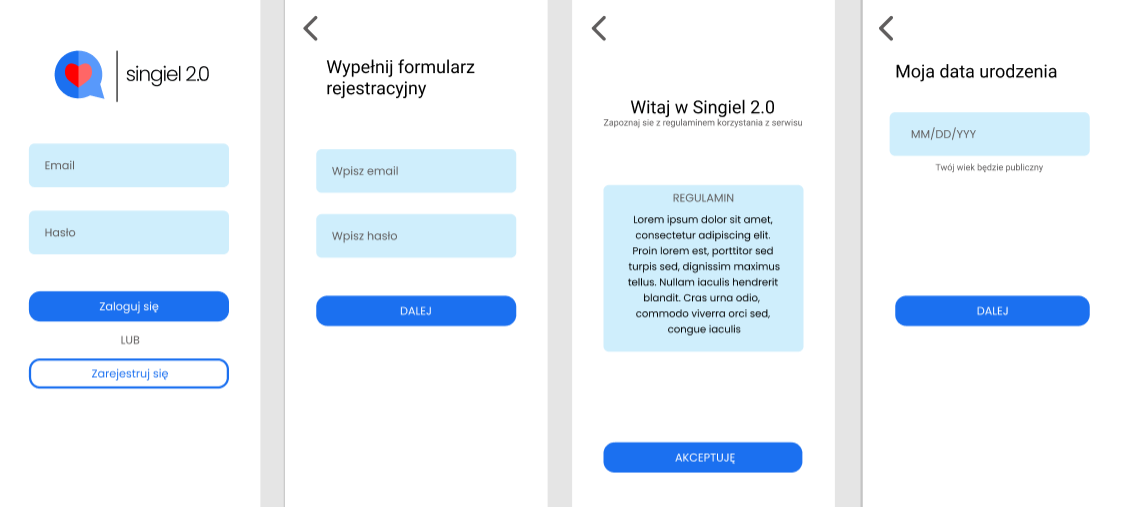
\includegraphics[width=14cm]{zdjęcia i skriny/log1.PNG}
\caption{Rejestracja i logowanie}
\end{figure}

\begin{figure}[h]
\centering
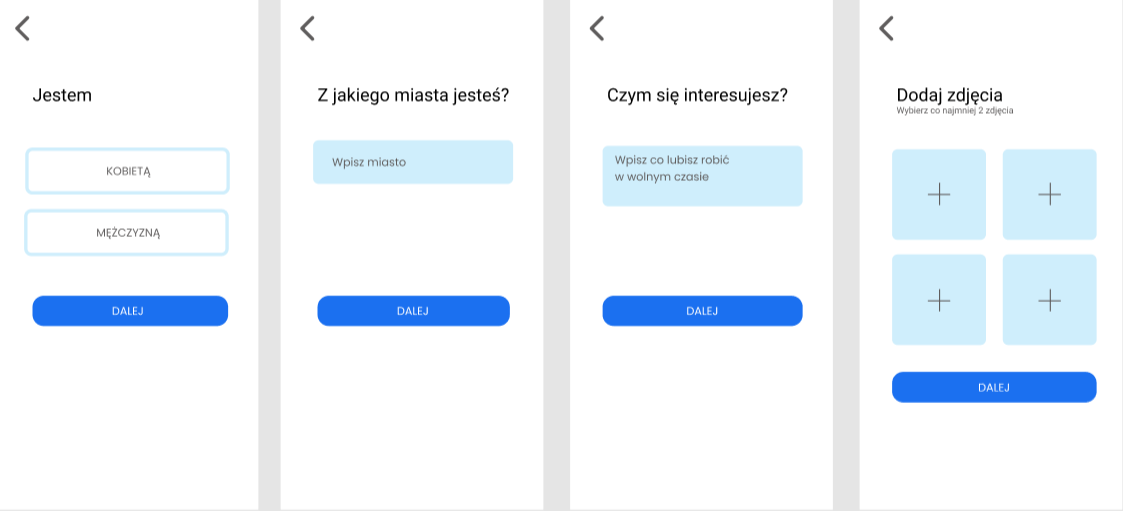
\includegraphics[width=14cm]{zdjęcia i skriny/log2.PNG}
\caption{Rejestracja i logowanie}
\end{figure}

\begin{figure}[htbp]
\centering
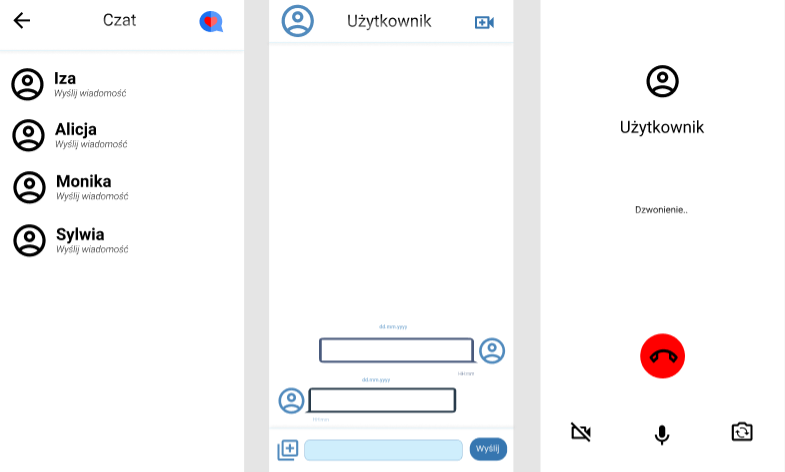
\includegraphics[width=15cm]{zdjęcia i skriny/czat1.PNG}
\caption{Czatowanie i wideo rozmowa}
\end{figure}

\begin{figure}[htbp]
\centering
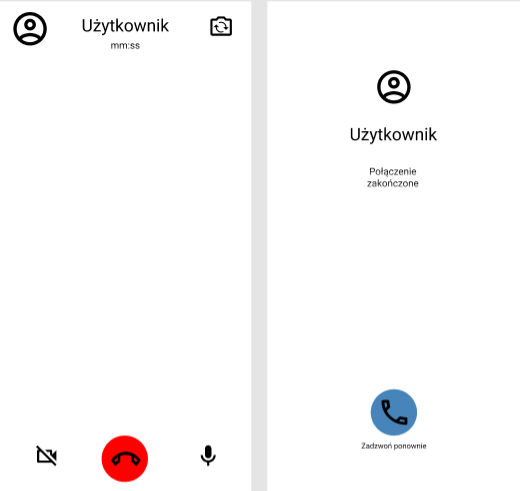
\includegraphics[width=10cm]{zdjęcia i skriny/czat2.PNG}
\caption{Czatowanie i wideo rozmowa}
\end{figure}
\begin{figure}[htbp]
\centering
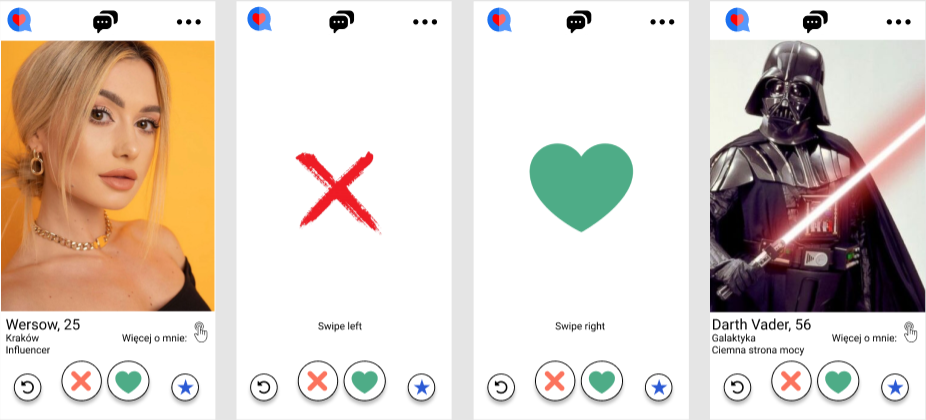
\includegraphics[width=15cm]{zdjęcia i skriny/swipe up.PNG}
\caption{Swipe up}
\end{figure}

\begin{figure}[h]
\centering
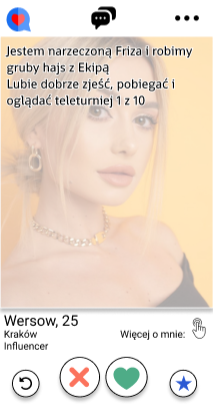
\includegraphics[width=5cm]{zdjęcia i skriny/swipe 2.PNG}
\caption{Opis użytkownika}
\end{figure}


\begin{figure}[h]
\centering
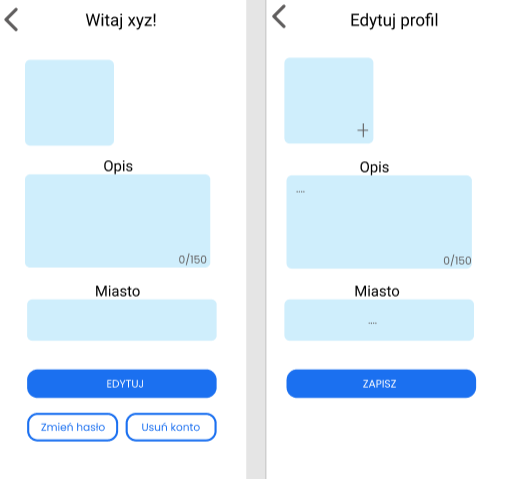
\includegraphics[width=9cm]{zdjęcia i skriny/edycja.PNG}
\caption{Edycja profilu}
\end{figure}


\end{document}